
%(BEGIN_QUESTION)
% Copyright 2008, Tony R. Kuphaldt, released under the Creative Commons Attribution License (v 1.0)
% This means you may do almost anything with this work of mine, so long as you give me proper credit

In electronics, we often plot the {\it characteristic curve set} for a transistor to show how it regulates current across a range of supply voltages.  This set of graphs proves useful in determining how the transistor will function in a real circuit:

$$\includegraphics[width=15.5cm]{i03226x01.eps}$$

We may do the same thing for a control valve, plotting a set of ``characteristic curves'' showing how it will restrict fluid flow across a range of pressure drops.  As with the transistor, this set of graphs proves useful in determining how the control valve will function in a real fluid system.

The following table shows this relationship for a linear control valve with a (maximum) $C_v$ of 18:

% No blank lines allowed between lines of an \halign structure!
% I use comments (%) instead, so that TeX doesn't choke.

$$\vbox{\offinterlineskip
\halign{\strut
\vrule \quad\hfil # \ \hfil & 
\vrule \quad\hfil # \ \hfil \vrule \cr
\noalign{\hrule}
%
% First row
Opening & $C_v$ \cr
%
\noalign{\hrule}
%
% Another row
0\% & 0 \cr
%
\noalign{\hrule}
%
% Another row
25\% & 4.5 \cr
%
\noalign{\hrule}
%
% Another row
50\% & 9 \cr
%
\noalign{\hrule}
%
% Another row
75\% & 13.5 \cr
%
\noalign{\hrule}
%
% Another row
100\% & 18 \cr
%
\noalign{\hrule}
} % End of \halign 
}$$ % End of \vbox

Use this valve's $C_v$ data, along with the equation relating flow ($Q$), pressure drop ($\Delta P$), specific gravity ($G_f$), and $C_v$ to plot a set of characteristic curves, one curve for each $C_v$ value shown in the table.  Assume that the fluid in question is water ($G_f$ = 1):

$$\includegraphics[width=15.5cm]{i03226x02.eps}$$

\underbar{file i03226}
%(END_QUESTION)





%(BEGIN_ANSWER)

$$\includegraphics[width=15.5cm]{i03226x03.eps}$$
 
%(END_ANSWER)





%(BEGIN_NOTES)


%INDEX% Electronics review: load lines
%INDEX% Final Control Elements, valve: characterization

%(END_NOTES)


